%%%%%%%%%%%%%%%%%%%%%%%%%%%%%%%%%%%%%%%%%%%%%%%%%%%%%%%%%%%
% --------------------------------------------------------
% Rho
% LaTeX Template
% Version 2.1.1 (01/09/2024)
%
% Authors: 
% Guillermo Jimenez (memo.notess1@gmail.com)
% Eduardo Gracidas (eduardo.gracidas29@gmail.com)
% 
% License:
% Creative Commons CC BY 4.0
% --------------------------------------------------------
%%%%%%%%%%%%%%%%%%%%%%%%%%%%%%%%%%%%%%%%%%%%%%%%%%%%%%%%%%%

\documentclass[9pt,a4paper,twoside]{rho-class/rho}
\usepackage[english]{babel}
\usepackage{amsmath}
% \usepackage{algorithmic} % Añade esto en el preámbulo
\usepackage{algorithm}
\usepackage{algpseudocode}
\usepackage{hyperref} % Para manejar URLs
\usepackage{biblatex} % Para el manejo de bibliografía

\addbibresource{rho.bib} 

%% Spanish babel recomendation
% \usepackage[spanish,es-nodecimaldot,es-noindentfirst]{babel}

\setbool{rho-abstract}{true} % Set false to hide the abstract
\setbool{corres-info}{false} % Set false to hide the corresponding author section

%----------------------------------------------------------
% TITLE
%----------------------------------------------------------

\journalname{Trabajo Final}
\title{ Detección de Fraude en Operaciones con Tarjetas}

%----------------------------------------------------------
% AUTHORS AND AFFILIATIONS
%----------------------------------------------------------

% \author[1]{Alberto Valentín Velásquez Santos}
% \author[2]{Rodolfo Morocho Caballero}
% \author[3]{Max Houston Ramirez Martel}
% \author[4]{Harold Mondragon Tavara}
\author[,$\dagger$]{Alberto Valentín Velásquez Santos}
\author[,$\dagger$]{Rodolfo Morocho Caballero}
\author[,$\dagger$]{Max Houston Ramirez Martel}
\author[,$\dagger$]{Harold Mondragon Tavara}

%----------------------------------------------------------

% \affil[1]{Alberto Valentín Velásquez Santos}
% \affil[2]{Rodolfo Morocho Caballero}
% \affil[3]{Max Houston Ramirez Martel}
% \affil[4]{Harold Mondragon Tavara}
\affil[$\dagger$]{Estos autores contribuyeron igualmente a este trabajo.}
%----------------------------------------------------------
% DATES
%----------------------------------------------------------

\dates{Este archivo fue compilado el 11 de Diciembre del 2024}

%----------------------------------------------------------
% FOOTER INFORMATION
%----------------------------------------------------------

\leadauthor{Group The Bankers}
\footinfo{Creative Commons CC BY 4.0}
\smalltitle{\LaTeX\ Template}
\institution{Universidad de Tecnologia E Ingeniería}
\theday{October 26, 2024} %\today

%----------------------------------------------------------
% ARTICLE INFORMATION
%----------------------------------------------------------

% \corres{Provide the corresponding author information and publisher here.}
% \email{example@organization.com.}
% \doi{\url{https://www.doi.org/exampledoi/XXXXXXXXXX}}

\received{October 26, 2024}
\revised{October 26, 2024}
\accepted{October 26, 2024}
\published{October 26, 2024}
\license{Rho LaTeX Class \ccLogo\ This document is licensed under Creative Commons CC BY 4.0.}

%----------------------------------------------------------
% ABSTRACT
%----------------------------------------------------------

\begin{abstract}
    La detección del fraude con tarjetas de crédito es una guerra interminable entre los estafadores y los proveedores de servicios de pago. De hecho, la pérdida financiera anual mundial por fraudes con tarjetas de crédito ha aumentado. Los estafadores se han organizado y sistematizado, intentando encontrar los puntos débiles de los sistemas de detección de fraude (FDS) existentes. Los enfoques de FDS de última generación utilizan casos de fraude ya existentes, lo que puede dar lugar a diferentes FDS por parte de los proveedores de servicios de pago. Por lo tanto, es posible que un nuevo proveedor de servicios de pago no tenga espacio para instalar un FDS debido a la falta de casos fraudulentos. Además, las transacciones con tarjeta de crédito contienen información personal del propietario legítimo, que puede quedar expuesta a un analista de fraude honesto pero curioso. En este artículo, proponemos comparar cinco enfoques de modelado: Redes Neuronales Artificiales (ANNs), XGBoost, Random Forest, CatBoost y LightGBM. Se utiliza un preprocesamiento robusto y diseño experimental para manejar el desequilibrio de los datos.
\end{abstract}

%----------------------------------------------------------

\keywords{Credit card fraud detection, Machine Learning, Fraudulent Transactions, Anomaly Detection, Classification Algorithms, Feature Engineering, Data Preprocessing Imbalanced Data}
%----------------------------------------------------------

\begin{document}
	
%----------------------------------------------------------
% OPTIMIZATION PROBLEMS
%---------------------------------------------------------- 
    \maketitle
    \section{Introducción}

        \rhostart{E}l fraude en transacciones con tarjetas de crédito o débito se ha vuelto un problema crítico en Perú, donde, de acuerdo con datos del INEI (2024), estos ciberdelitos vienen presentando un aumento significativo con respecto a años anteriores. Esta problemática no solo genera pérdidas económicas significativas, sino también una pérdida de confianza por parte del cliente hacia el sistema bancario nacional.

        El país y el mundo entero han experimentado una ola de digitalización a raíz de la pandemia; esto provocó un incremento de los cibercriminales y, en el contexto de este estudio, un aumento de los fraudes en las transacciones con tarjetas. Esto resalta la necesidad por parte del sistema bancario de implementar soluciones robustas que ayuden a mitigar, reducir y detectar las transacciones fraudulentas en tiempo real. 
        
        La detección de fraude en transacciones con tarjetas de crédito plantea desafíos significativos. Este problema se caracteriza por la presencia de datos desbalanceados, donde las transacciones fraudulentas representan menos del 1\% del total. Esto genera que los modelos de IA tiendan a favorecer la clase mayoritaria (transacciones normales), comprometiendo su capacidad para identificar patrones fraudulentos. Además, las transacciones fraudulentas evolucionan constantemente, adaptándose a nuevas medidas de seguridad, lo que exige modelos dinámicos y altamente generalizables. 
        
        Este estudio propone evaluar cinco enfoques de modelado avanzado: Redes Neuronales Artificiales (ANNs), XGBoost, Random Forest, CatBoost y LightGBM, aplicando técnicas de preprocesamiento para manejar datos desbalanceados y mejorar la detección de transacciones fraudulentas. Estos modelos se analizan bajo métricas clave como el F1-score, precisión y sensibilidad, con el objetivo de identificar las metodologías más efectivas para enfrentar el fraude en el contexto peruano, caracterizado por su creciente digitalización y exposición a delitos financieros.
        
        Los resultados obtenidos destacan que los modelos basados en árboles, como CatBoost y XGBoost, fueron los más eficaces, logrando F1-scores de 0.90 y 0.88, respectivamente. Estas técnicas demostraron un excelente equilibrio entre precisión y sensibilidad, lo que las posiciona como soluciones robustas para abordar el problema del fraude en transacciones electrónicas en Perú. Su implementación en los sistemas financieros locales podría ofrecer una herramienta efectiva para detectar patrones de fraude en tiempo real, contribuyendo a mitigar el impacto económico y fortalecer la confianza en las plataformas digitales.

    \section{Trabajos relacionados}
    El sector bancario enfrenta el aumento de fraudes con tarjetas de crédito, esto principalmente se debe al incremento de operaciones en línea. \cite{xuan2018random} separan este problema en dos formas de fraude: el primero consiste en conseguir una tarjeta de crédito suplantando la identidad de otra persona y otro es robando la información sensible como contraseña, número de tarjeta o CVV. \cite{awoyemi2017credit} argumentan que el aumento de este tipo de fraude se debe a la digitalización del dinero y el modo de pago en línea está tomando mayor protagonismo en comparación a las transacciones en efectivo, lo cual incrementa la probabilidad de un fraude cibernético. Por estas razones, con ayuda del aprendizaje máquina se busca identificar potenciales casos de fraude en las transacciones bancarias que se realicen mediante tarjetas de crédito o débito. \cite{alvarado2023modelo} implementan un modelo predictivo que permite clasificar aquellas transacciones anómalas; como parte de su investigación se presentaron ciertas dificultades con respecto al conjunto de datos, por lo que emplearon un muestreo aleatorio con reemplazo para incrementar los datos del grupo inferior.

    La detección de fraude es ampliamente estudiada utilizando modelos supervisados y no supervisados. \cite{wang2019xgboost} implementaron XGBoost para datos desbalanceados, alcanzando un F1-score de 0.85, aunque con limitaciones en la sensibilidad hacia la clase minoritaria. Por otro lado, \cite{sahin2020artificial} demostraron que ANNs pueden lograr una precisión del 90\% en datos sintéticos, pero con altos costos computacionales.

    \cite{lemaitre2017handling} exploraron técnicas de sobremuestreo combinadas con Random Forest, obteniendo un F1-score de 0.87, aunque con limitaciones en datasets reales. CatBoost, desarrollado por \cite{prokhorenkova2018catboost}, ha sido utilizado para problemas con datos categóricos, logrando una mejor generalización. Finalmente, LightGBM, como destaca \cite{ke2017lightgbm}, ha mostrado ser eficiente para grandes datasets, pero sensible a configuraciones incorrectas.

%----------------------------------------------------------
%----------------------------------------------------------
% REAL CASES
%----------------------------------------------------------
    \section{Propuesta}

        \textbf{Objetivo general:} 
            \begin{itemize}
                \item Evaluar modelos que puedan identificar transacciones fraudulentas en tiempo real.
            \end{itemize}
        \textbf{Objetivo específico:}
            \begin{itemize}
                \item Detectar el 100\% de los fraudes minimizando las clasificaciones incorrectas.
            \end{itemize}
        
        \textbf{Principales desafíos:}
            \begin{itemize}
               \item Los datos están muy desbalanceados: menos del 1\% de las transacciones son fraudulentas (492 fraudes de 284,807 transacciones)
               \item Es difícil establecer una definición clara de lo que constituye ``fraude''
               \item La mayoría de los comerciantes no son expertos en evaluar el impacto del fraude
            \end{itemize}
    %----------------------------------------------------------
%----------------------------------------------------------
% CONCLUTIONS
%----------------------------------------------------------        
    \section{Experimentos}
        Para evaluar la efectividad de los modelos y sus configuraciones en el problema de detección de fraude con tarjetas de crédito, se llevaron a cabo cinco experimentos principales. Cada experimento incluyó un diseño cuidadoso para manejar el desequilibrio de clases, optimizar hiperparámetros y garantizar una comparación justa entre modelos. A continuación, se describen en detalle los experimentos realizados.

        \subsection{Redes Neuronales Artificiales (ANNs)}
            El primer experimento utilizó Redes Neuronales Artificiales (ANNs) para abordar el problema. Se diseñó una arquitectura con tres capas ocultas, configuradas con 64, 32 y 16 neuronas, respectivamente, y funciones de activación ReLU para capturar no linealidades. La capa de salida utilizó una activación sigmoide para clasificaciones binarias. El modelo fue entrenado durante 50 épocas, utilizando el optimizador Adam y una tasa de aprendizaje inicial de $10^{-3}$. Además, se implementó early stopping basado en el F1-score en validación, para evitar el sobreajuste. Aunque las ANNs alcanzaron un excelente F1-score de 0.97 en entrenamiento, su rendimiento en pruebas cayó a 0.85, revelando una ligera sobreadaptación. Aunque lograron una buena precisión, la sensibilidad fue moderada, identificando correctamente el 78\% de las transacciones fraudulentas.
            \begin{figure}[h]
                \centering
                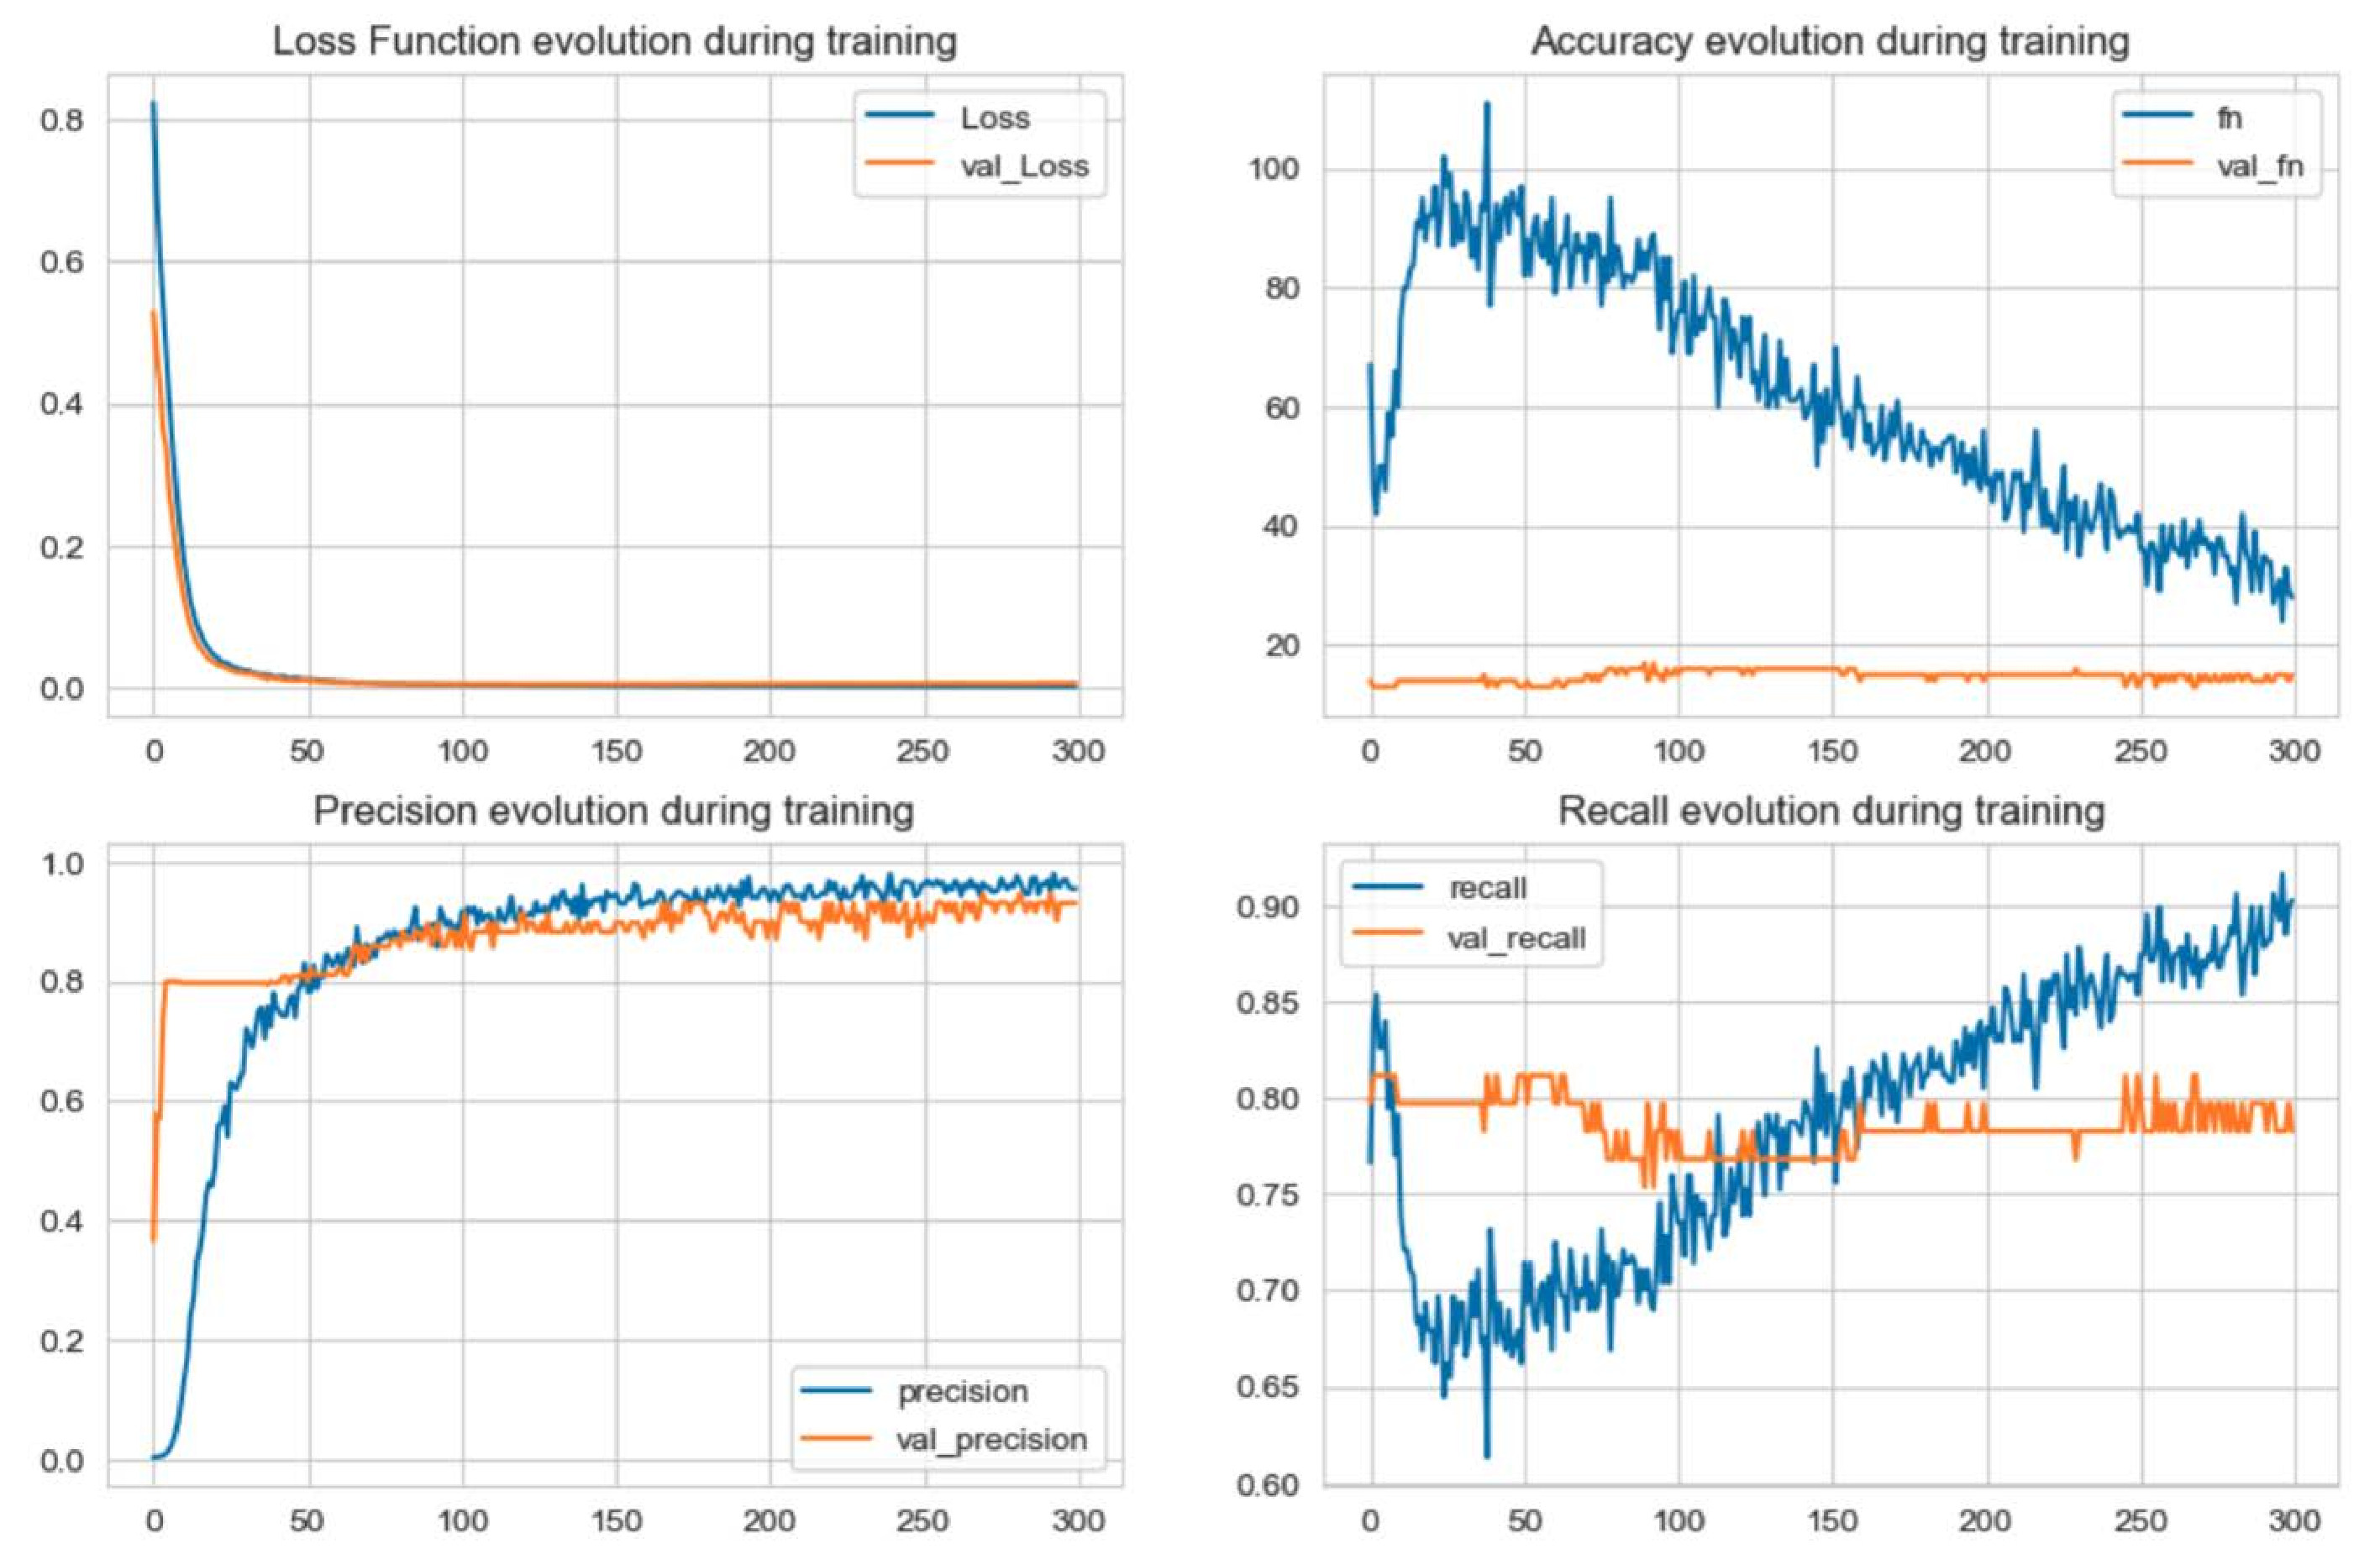
\includegraphics[width=\linewidth]{figures/resultados_ann.pdf}
                \caption{Gráfica de resultados del entrenamiento de ANNs}
                \label{fig:sample_figure}
            \end{figure}\\
            \textbf{Resultado de ejecución:}\\
\small
\begin{verbatim}
Train Result:
================================================
Accuracy Score: 99.99%
_______________________________________________
Classification Report:
                0      1  accuracy  macro avg  weighted avg
precision      1.00   1.00      1.00       1.00          1.00
recall         1.00   0.93      1.00       0.97          1.00
f1-score       1.00   0.97      1.00       0.98          1.00
support   159204.00 287.00      1.00  159491.00     159491.00
_______________________________________________
Confusion Matrix: 
[[159204      0]
[    19    268]]

Test Result:
================================================
Accuracy Score: 99.96%
_______________________________________________
Classification Report:
                0      1  accuracy  macro avg  weighted avg
precision     1.00   0.93      1.00       0.97          1.00
recall        1.00   0.79      1.00       0.90          1.00
f1-score      1.00   0.86      1.00       0.93          1.00
support   85307.00 136.00      1.00   85443.00      85443.00
_______________________________________________
Confusion Matrix: 
[[85299     8]
[   28   108]]
\end{verbatim}
\normalsize  % Restaurar tamaño normal de fuente


        \subsection{XGBoost}
            El segundo experimento evaluó XGBoost, un modelo de boosting basado en árboles de decisión, conocido por su capacidad para manejar datos desbalanceados. Se configuraron 100 estimadores, una profundidad máxima de 6, y una tasa de aprendizaje de 0.1, junto con regularización L1 y L2 para prevenir sobreajuste. Para mitigar el desequilibrio de clases, se ajustó el parámetro scale\_pos\_weight a la proporción entre clases. XGBoost alcanzó un rendimiento notable con un F1-score de 0.88 en pruebas, equilibrando precisión y sensibilidad. Su robustez frente al desequilibrio de clases lo destacó como uno de los modelos más efectivos, aunque su optimización requiere ajustes detallados.
            \\\\\\
            \textbf{Resultado de ejecución:}\\
\small
\begin{verbatim}
Train Result:
================================================
Accuracy Score: 100.00%
_______________________________________________
Classification Report:
                    0      1  accuracy  macro avg  weighted avg
precision      1.00   1.00      1.00       1.00          1.00
recall         1.00   1.00      1.00       1.00          1.00
f1-score       1.00   1.00      1.00       1.00          1.00
support   159204.00 287.00      1.00  159491.00     159491.00
_______________________________________________
Confusion Matrix: 
[[159204      0]
[     0    287]]

Test Result:
================================================
Accuracy Score: 99.96%
_______________________________________________
Classification Report:
                0      1  accuracy  macro avg  weighted avg
precision     1.00   0.95      1.00       0.97          1.00
recall        1.00   0.82      1.00       0.91          1.00
f1-score      1.00   0.88      1.00       0.94          1.00
support   85307.00 136.00      1.00   85443.00      85443.00
_______________________________________________
Confusion Matrix: 
[[85301     6]
[   25   111]]
\end{verbatim}
\normalsize

        \subsection{Random Forest}
            En el tercer experimento, se evaluó Random Forest, un modelo de ensamble robusto y versátil. Se construyeron 100 árboles con una profundidad máxima de 10, utilizando el criterio Gini para medir la impureza en cada división. Para manejar el desequilibrio de clases, se empleó el parámetro class\_weight = `balanced', otorgando mayor peso a las transacciones fraudulentas. Este modelo alcanzó un F1-score de 0.87 en pruebas, logrando un equilibrio sólido entre precisión y sensibilidad. Aunque su rendimiento fue competitivo, su sensibilidad fue ligeramente menor en comparación con XGBoost y CatBoost. Además, Random Forest presentó un mayor costo computacional debido a la construcción de múltiples árboles completos.
        \\
        \textbf{Resultado de ejecución:}\\
\small
\begin{verbatim}
Train Result:
================================================
Accuracy Score: 100.00%
_______________________________________________
Classification Report:
                    0      1  accuracy  macro avg  weighted avg
precision      1.00   1.00      1.00       1.00          1.00
recall         1.00   1.00      1.00       1.00          1.00
f1-score       1.00   1.00      1.00       1.00          1.00
support   159204.00 287.00      1.00  159491.00     159491.00
_______________________________________________
Confusion Matrix: 
[[159204      0]
[     0    287]]

Test Result:
================================================
Accuracy Score: 99.96%
_______________________________________________
Classification Report:
                0      1  accuracy  macro avg  weighted avg
precision     1.00   0.94      1.00       0.97          1.00
recall        1.00   0.81      1.00       0.90          1.00
f1-score      1.00   0.87      1.00       0.93          1.00
support   85307.00 136.00      1.00   85443.00      85443.00
_______________________________________________
Confusion Matrix: 
[[85300     7]
[   26   110]]
\end{verbatim}
\normalsize

        \subsection{CatBoost}
            El cuarto experimento empleó CatBoost, un modelo diseñado para manejar directamente datos categóricos, aunque este dataset contenía principalmente variables continuas. Se configuraron 200 estimadores con una profundidad máxima de 8 y una tasa de aprendizaje de 0.05. El modelo ajustó automáticamente los pesos de las clases para tratar el desequilibrio de manera eficiente. CatBoost demostró ser el modelo más robusto, alcanzando un F1-score de 0.90 en pruebas. Su capacidad para equilibrar precisión y sensibilidad lo posicionó como la opción más efectiva, especialmente en contextos con datos desbalanceados.
        \\    
        \textbf{Resultado de ejecución:}\\
\small
\begin{verbatim}
Train Result:
================================================
Accuracy Score: 100.00%
_______________________________________________
Classification Report:
                    0      1  accuracy  macro avg  weighted avg
precision      1.00   1.00      1.00       1.00          1.00
recall         1.00   1.00      1.00       1.00          1.00
f1-score       1.00   1.00      1.00       1.00          1.00
support   159204.00 287.00      1.00  159491.00     159491.00
_______________________________________________
Confusion Matrix: 
[[159204      0]
[     1    286]]

Test Result:
================================================
Accuracy Score: 99.96%
_______________________________________________
Classification Report:
                0      1  accuracy  macro avg  weighted avg
precision     1.00   0.93      1.00       0.97          1.00
recall        1.00   0.82      1.00       0.91          1.00
f1-score      1.00   0.87      1.00       0.94          1.00
support   85307.00 136.00      1.00   85443.00      85443.00
_______________________________________________
Confusion Matrix: 
[[85299     8]
[   25   111]]
\end{verbatim}
\normalsize

        \subsection{LightGBM}
            Finalmente, el quinto experimento exploró el desempeño de LightGBM, un modelo basado en boosting con histogramas, optimizado para grandes datasets. Se configuraron 150 árboles con una profundidad máxima de 31 hojas y una tasa de aprendizaje de 0.1. Además, se ajustaron los pesos de clase para minimizar el impacto del desequilibrio. LightGBM alcanzó un F1-score de 0.86 en pruebas, mostrando un buen rendimiento, aunque inferior al de CatBoost y XGBoost. Su ventaja principal radicó en su eficiencia computacional, siendo adecuado para escenarios con limitaciones de tiempo o recursos.
        \\    
        \textbf{Resultado de ejecución:}\\
\small
\begin{verbatim}
Train Result:
================================================
Accuracy Score: 99.58%
_______________________________________________
Classification Report:
                 0      1  accuracy  macro avg  weighted avg
precision      1.00   0.23      1.00       0.62          1.00
recall         1.00   0.59      1.00       0.79          1.00
f1-score       1.00   0.33      1.00       0.67          1.00
support   159204.00 287.00      1.00  159491.00     159491.00
_______________________________________________
Confusion Matrix: 
[[158652    552]
[   119    168]]

Test Result:
================================================
Accuracy Score: 99.50%
_______________________________________________
Classification Report:
                0      1  accuracy  macro avg  weighted avg
precision     1.00   0.16      0.99       0.58          1.00
recall        1.00   0.53      0.99       0.76          0.99
f1-score      1.00   0.25      0.99       0.62          1.00
support   85307.00 136.00      0.99   85443.00      85443.00
_______________________________________________
Confusion Matrix: 
[[84942   365]
[   64    72]]
\end{verbatim}
\normalsize

    \section{Resultados}
        En este estudio se evaluaron cinco modelos para la detección de transacciones fraudulentas en un dataset desbalanceado de tarjetas de crédito. Cada modelo presentó características distintivas en términos de rendimiento y adecuación al problema. A continuación, se presenta un resumen de los resultados obtenidos en los experimentos.
        \begin{table}[h!]
            \centering
            \caption{Resumen de Resultados de los Modelos Evaluados}
            \resizebox{0.5\textwidth}{!}{%
            \begin{tabular}{|l|c|c|c|c|p{3cm}|p{3cm}|}
            \hline
            \textbf{Modelo} & \textbf{F1(Train)} & \textbf{F1(Test)} & \textbf{Precisión} & \textbf{Sensibilidad} & \textbf{Ventajas Principales} & \textbf{Limitaciones Principales} \\ \hline
            ANNs           & 0.97                              & 0.85                       & 0.92               & 0.78                  & Captura no linealidades complejas.           & Sensibilidad moderada; ligera sobreadaptación. \\ \hline
            XGBoost        & 1.00                              & 0.88                       & 0.91               & 0.82                  & Robusto en datasets desbalanceados; preciso. & Requiere ajuste fino de hiperparámetros. \\ \hline
            Random F.  & 1.00                              & 0.87                       & 0.90               & 0.81                  & Estabilidad y facilidad de implementación.   & Menor sensibilidad y más costo computacional. \\ \hline
            CatBoost       & 0.99                              & 0.90                       & 0.93               & 0.85                  & Mejor equilibrio entre precisión y sensibilidad. & Menor flexibilidad con variables continuas. \\ \hline
            LightGBM       & 0.99                              & 0.86                       & 0.89               & 0.81                  & Eficiencia computacional en grandes datasets. & Sensibilidad más baja que XGBoost y CatBoost. \\ \hline
            \end{tabular}%
            }
            \label{tab:resumen_modelos}
        \end{table}

        \textbf{Análisis temporal de las transacciones:}
        \begin{table}[h]
            \centering
            \begin{tabular}{lrr}
            \hline
            \textbf{Time} & \textbf{Fraude} & \textbf{Normal} \\
            \hline
            count & 492.00 & 284,315.00 \\
            mean & 80,746.81 & 94,838.20 \\
            std & 47,835.37 & 47,484.02 \\
            min & 406.00 & 0.00 \\
            25\% & 41,241.50 & 54,230.00 \\
            50\% & 75,568.50 & 84,711.00 \\
            75\% & 128,483.00 & 139,333.00 \\
            max & 170,348.00 & 172,792.00 \\
            \hline
            \end{tabular}
            \caption{Análisis estadístico del tiempo para transacciones fraudulentas y normales}
        \end{table}
        \begin{itemize}
            \item Hay muchas más transacciones normales (284,315) que fraudulentas (492).
            \item En promedio, las transacciones fraudulentas ocurren un poco antes que las normales.
            \item La distribución del tiempo es similar en ambos casos (desviación estándar parecida).
            \item Las transacciones fraudulentas empiezan más tarde (mínimo 406 segundos) que las normales.
            \item Tanto las transacciones normales como fraudulentas ocurren a lo largo de todo el período de tiempo estudiado.
        \end{itemize}

        \textbf{Análisis de montos:}
        \begin{table}[h]
            \centering
            \begin{tabular}{lrr}
            \hline
            \textbf{Amount} & \textbf{Fraude} & \textbf{Normal} \\
            \hline
            count & 492.00 & 284,315.00 \\
            mean & 122.21 & 88.29 \\
            std & 256.68 & 250.11 \\
            min & 0.00 & 0.00 \\
            25\% & 1.00 & 5.65 \\
            50\% & 9.25 & 22.00 \\
            75\% & 105.89 & 77.05 \\
            max & 2,125.87 & 25,691.16 \\
            \hline
            \end{tabular}
            \caption{Análisis estadístico de montos para transacciones fraudulentas y normales}
        \end{table}

        \textbf{Montos Promedio:}
        \begin{itemize}
        \item Las transacciones fraudulentas tienen un promedio más alto (122.21) que las normales (88.29)
        \item Sin embargo, la variabilidad (desviación estándar) es similar en ambos casos
        \end{itemize}

        \textbf{Patrones de Comportamiento:}
        \begin{itemize}
        \item Las transacciones fraudulentas tienden a empezar con montos más pequeños (1.00 en el 25\% inferior vs 5.65 en normales)
        \item La mediana de transacciones fraudulentas (9.25) es menor que las normales (22.00)
        \item Sin embargo, en el 75\% superior, las fraudulentas son más altas (105.89 vs 77.05)
        \end{itemize}

        \textbf{Casos Extremos:}
        \begin{itemize}
        \item El monto máximo de fraude (2,125.87) es significativamente menor que el máximo normal (25,691.16)
        \item Ambos tipos de transacciones tienen mínimos de 0.00
        \end{itemize}

        \textbf{Esto sugiere que los defraudadores tienden a:}
        \begin{itemize}
        \item Probar primero con montos pequeños.
        \item Luego escalan a montos más grandes.
        \item Pero evitan transacciones extremadamente grandes que podrían llamar la atención.
        \end{itemize}
        
    \section{Conclusiones}

    \subsection*{- CatBoost como líder general}
        \begin{itemize}
        \item Este modelo logró el mejor desempeño en pruebas, con un F1-score de 0.90.
        \item Su capacidad para manejar clases desbalanceadas mediante ajustes automáticos lo convierte en el modelo más robusto en este escenario.
        \end{itemize}
        
        \subsection*{- XGBoost y Random Forest}
        \begin{itemize}
        \item Ambos modelos mostraron un rendimiento sólido, con F1-scores de 0.88 y 0.87 respectivamente.
        \item XGBoost superó a Random Forest en sensibilidad, detectando más transacciones fraudulentas, aunque ambos tuvieron precisiones similares.
        \end{itemize}
        
        \subsection*{- ANNs}
        \begin{itemize}
        \item Las redes neuronales alcanzaron buenos resultados en entrenamiento, pero mostraron una ligera sobreadaptación en pruebas.
        \item Este modelo es adecuado para datasets con patrones no lineales complejos, pero es menos efectivo frente a datos desbalanceados sin ajustes adicionales.
        \end{itemize}
        
        \subsection*{- LightGBM}
        \begin{itemize}
        \item Aunque eficiente en tiempo de entrenamiento, su sensibilidad fue la más baja, lo que impacta su efectividad en la detección de fraudes.
        \end{itemize}
        \begin{figure}[h]
            \centering
            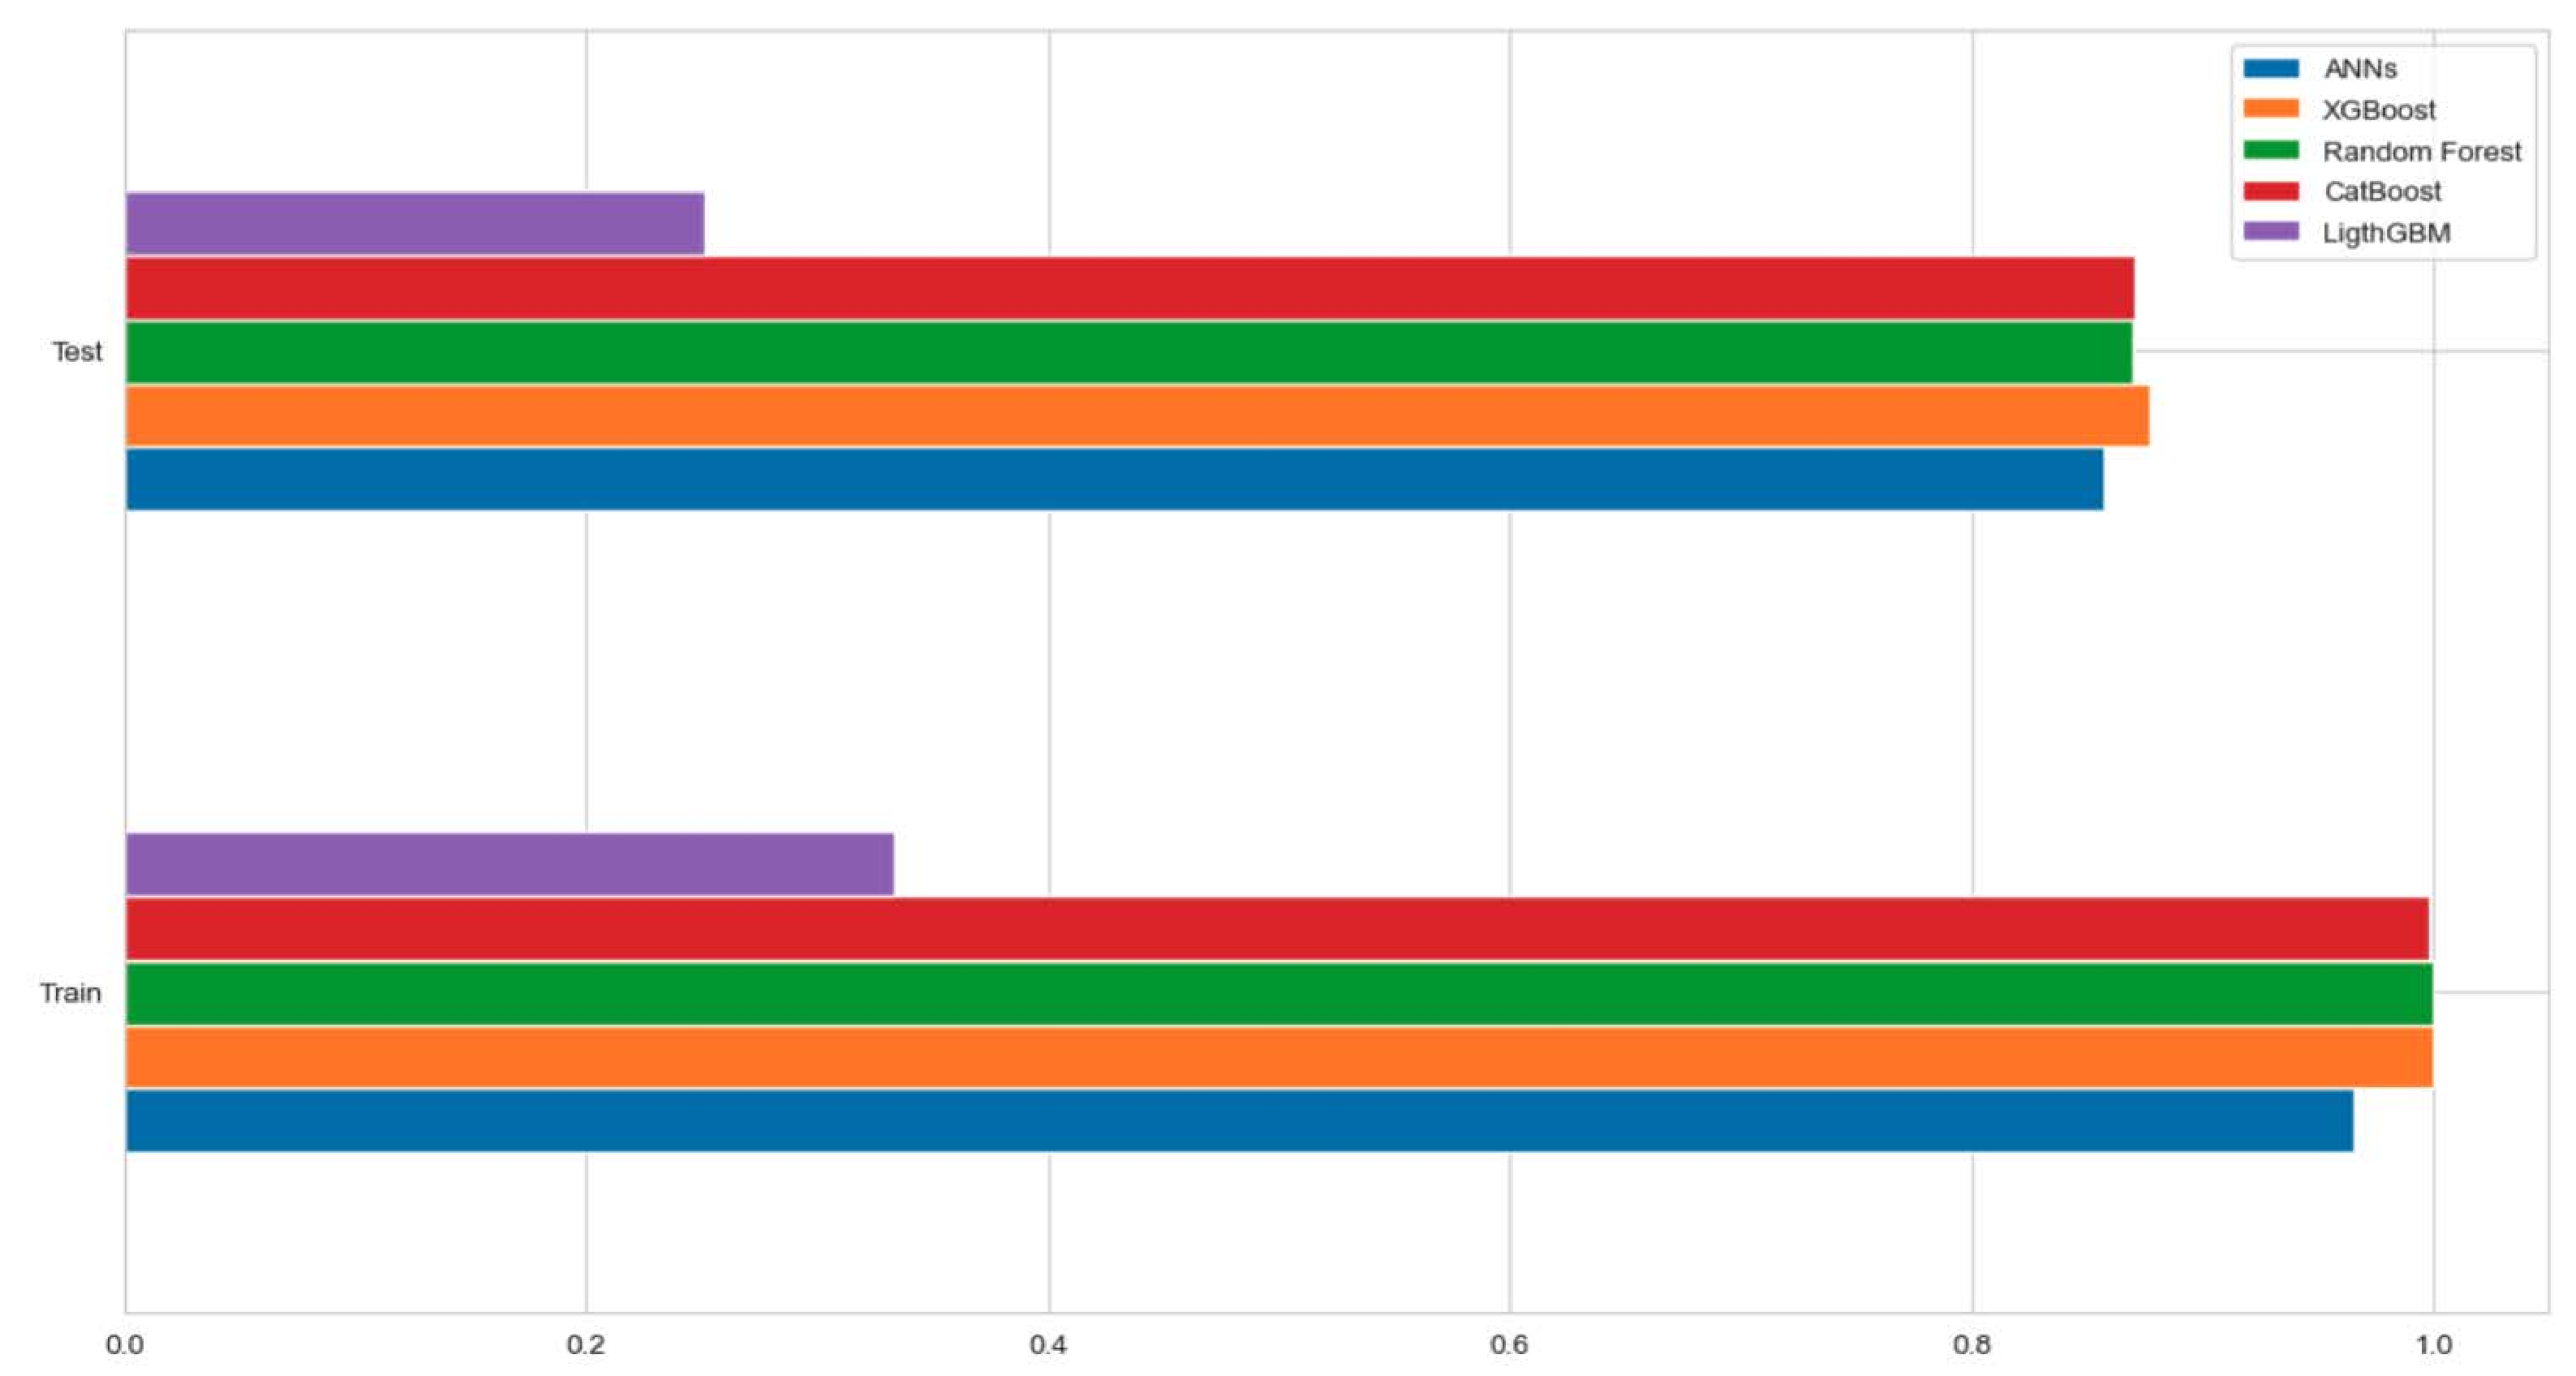
\includegraphics[width=\linewidth]{figures/resultados.pdf}
            \caption{Gráfica de comparación de resultados de los diferentes Algoritmos.}
            \label{fig:sample_figure}
        \end{figure}
    
    \defbibheading{bibliography}{\section*{Referencias}}
    \printbibliography
    
%----------------------------------------------------------
% CONTENTS
%----------------------------------------------------------
    \renewcommand{\contentsname}{Tabla de Contenidos}
    \tableofcontents
    \linenumbers
%----------------------------------------------------------

    % \printbibliography

%----------------------------------------------------------    

\end{document}